\documentclass[conference]{IEEEtran}
\IEEEoverridecommandlockouts

\usepackage{cite}
\usepackage{amsmath,amssymb}
\usepackage{graphicx}
\graphicspath{{../figures/}{figures/}}
\usepackage{booktabs}
\usepackage{array}
\newcolumntype{L}[1]{>{\raggedright\arraybackslash}p{#1}}
\usepackage{multirow}
\usepackage{xcolor}
\usepackage{tikz}
\usetikzlibrary{arrows.meta,positioning,fit,calc}
\usepackage[hidelinks]{hyperref}
\usepackage{microtype}

\newcommand{\authorname}{Tancrède Amiel}
\newcommand{\repourl}{https://github.com/TancredeA/autogear-embedded-ml}
\newcommand{\vhat}{\hat{v}}
\newcommand{\lhat}{\hat{\ell}}
\newcommand{\pct}{\,\%}

\begin{document}

\title{Learning to Shift Without a Torque Sensor:\\ A Data-Driven Extension of the AutoGear\\ Automatic Derailleur Project}

\author{\IEEEauthorblockN{\authorname}
\IEEEauthorblockA{CentraleSupélec, entrepreneurship track\\ Extension of the AutoGear project (Shifter Pro), October 2026}}

\maketitle

\begin{abstract}
During AutoGear, a student project of the CentraleSupélec entrepreneurship track, my team and I designed the Shifter Pro, a low-cost device that turns the derailleur of an ordinary bicycle into an automatic one. Its decision logic must choose gears without a torque sensor and run on an Arduino-class microcontroller. The rides the prototype was meant to record could not be collected before the project ended, so this study rebuilds their closest public equivalent: 18.9~hours of one-second data by six cyclists, restricted to quantities the device can compute, with the rider's gear recovered from the speed-to-cadence ratio and checked against real Di2 shift data (84\pct{} of pedalling seconds correct). The formulation first planned, classifying shift events second by second, faces class imbalance (2.6\pct{} of seconds), ambiguous timing and closed-loop drift; in closed-loop replay it agrees with the rider within one gear only 66.0\pct{} of the time, below a constant-cadence decision table. I instead regress the development of the gear the rider will want a few seconds ahead from 14 inputs that do not depend on the engaged gear, and leave shift timing to a hysteresis controller. With 100 boosted trees, the policy agrees with the rider within one gear 87.0\pct{} of the time, against 80.8\pct{} for a decision table given the pedalling torque; it wins 13 of 14 within-rider tests, shifts as often as the rider and almost never reverses a shift, but loses this advantage when trained on other riders. A 172-byte linear regression of the same target already beats every decision table, so the reformulation carries most of the gain. Exported to C, the model and controller fit in 14.9~KB of flash and 316~bytes of state on a Cortex-M4F, and reproduce the Python reference exactly. The results suggest that the learned policy chooses gears better than a decision table; they rest on reconstructed labels and a simulated closed loop, so without a field test they establish feasibility, not on-bike performance.
\end{abstract}

\begin{IEEEkeywords}
automatic gear shifting, embedded machine learning, imitation learning, gradient boosting, class imbalance, closed-loop evaluation, microcontrollers
\end{IEEEkeywords}

% =====================================================================================
\section{Introduction}
% =====================================================================================

\subsection{The AutoGear project and the Shifter Pro}
The Shifter Pro is the product my team and I developed during AutoGear, a four-student project of the CentraleSupélec entrepreneurship track (January 2025 to June 2026): a retrofit device that turns the derailleur of a conventional bicycle into an automatic one. A servomotor moves the cable, and an embedded Arduino controller decides when to shift. The intended users are urban and occasional cyclists, for whom constant gear management is a source of fatigue and hesitation. The product sits between a plain mechanical bicycle and an e-bike: it should offer some of the ease of the latter at a fraction of its price.

The decision logic we had in mind was to imitate an experienced cyclist. Rather than hard-coding thresholds, the device would learn from demonstrations of how a skilled rider shifts, with the longer-term prospect of adapting to each user. Commercial systems move in the same direction: Shimano's Q'AUTO decides from speed, cadence and slope, and adjusts its behaviour to the rider's manual corrections~\cite{qauto}.

To collect those demonstrations, my team and I built several mechanical prototypes of the Shifter Pro, the last of which was designed to record ride data: the plan was to ride it across town and log our own shifting, so that the model would learn from our riding. That database was to be the basis for training the decision model, turning the mechanical device into an intelligent one. Lack of time and bad weather prevented us from ever making those recordings.

\subsection{Design constraints}
Four constraints, all following from the price target, shape what the decision logic can use and how large it can be.

\textbf{C1. No torque sensor.} A pedalling-torque sensor is the most direct measure of rider effort, but also one of the most expensive components of an automatic drivetrain. Leaving it out is the premise of the product.

\textbf{C2. Only the prototype's sensors.} The controller is an Arduino Nano 33 BLE Sense Rev2, whose board carries a 6-axis IMU (BMI270) and a barometer (LPS22HB)~\cite{nano}, plus a Hall-effect cadence sensor on the crank. There is no GPS and no wheel-speed sensor; the engaged gear is known because the device sets it.

\textbf{C3. Embedded inference.} The nRF52840 microcontroller offers a 64~MHz Cortex-M4F, 1~MB of flash and 256~KB of RAM. The decision model must fit in tens of kilobytes, run in well under a millisecond and need no machine-learning runtime.

\textbf{C4. Mechanical rules.} One decision every 0.5 to 1~s, at most one gear step at a time, and no shift while coasting, since the chain must turn for the derailleur to act.

\subsection{Research question}\label{sec:question}
The planned recordings never took place, and the prototype is no longer available: neither data collection nor on-bike testing is possible. The question the prototype was meant to answer therefore remains open, and it is the subject of this study, carried out after the project as a proof of concept. Without a torque sensor, the natural solution, a decision table with thresholds on cadence and effort, cannot be written, because effort is not measured. The question is:

\begin{quote}
\emph{Can a statistical model, fed only with what the prototype measures in real time, make better gear decisions than such a table, even when the table is given the torque the product does without?}
\end{quote}

\subsection{Difficulties}\label{sec:difficulties}
The rest of the study is organised around eight difficulties; each design choice below refers back to them.

\textbf{D1. Partial observability.} Effort is not measured (C1). Two situations with the same cadence, speed and slope can call for different gears, depending on how hard the rider pushes; whatever is missing must be inferred from the recent history of the observable signals.

\textbf{D2. Rare decisions.} A rider shifts on a small fraction of seconds: 2.6\pct{} in the data used here, one shift every 38~s. Any formulation that predicts shifts directly faces a strong class imbalance.

\textbf{D3. Ambiguous timing.} For a given situation there is a window of acceptable instants to shift, not a single correct second. Per-second labels therefore carry timing noise that no model can remove.

\textbf{D4. Closed loop.} The gear the policy selects changes the cadence it observes next. Accuracy measured offline on the rider's own trajectory does not tell how the policy behaves once its own choices feed back into its inputs.

\textbf{D5. No first-party data.} The dataset the prototype would have recorded does not exist. It has to be rebuilt from public sources, keeping only quantities the device can compute, and the rider's gear has to be inferred.

\textbf{D6. Little data per rider.} Imitating a reference rider means learning from hours of that rider, not from thousands of riders.

\textbf{D7. Embedded budget.} The model must respect C3 and be exportable to plain C.

\textbf{D8. No prototype.} The policy cannot be tested on a bicycle; its closed-loop behaviour must be simulated.

\subsection{Contributions}
This study makes five contributions. (i)~It assembles a public dataset restricted to device-accessible quantities, with gear labels validated on real electronic-shifting data (Section~\ref{sec:data}). (ii)~It defines a closed-loop replay protocol that measures how a policy rides, not only how it predicts (Section~\ref{sec:protocol}). (iii)~It shows why the formulation first planned, a two-stage classifier of shift events, falls short (Section~\ref{sec:event}). (iv)~It proposes a target-gear regression coupled with a hysteresis controller, and compares it with decision tables, with and without torque, and with other statistical models (Sections~\ref{sec:method} and~\ref{sec:results}). (v)~It implements the retained policy in plain C for the target microcontroller and verifies it against the reference implementation (Section~\ref{sec:embedded}). Code, data pipeline and firmware are available in the companion repository.

% =====================================================================================
\section{Related Work}
% =====================================================================================
\textbf{Automatic shifting.} Commercial automatic derailleurs decide from speed, cadence and slope and adapt to the rider's corrections~\cite{qauto}; on electric bicycles, rule-based and fuzzy controllers use motor or torque information~\cite{fuzzy}. Both rely on hand-designed rules whose inputs include effort, which is exactly what C1 removes.

\textbf{Imitation learning.} Learning a policy from demonstrations by supervised learning (behavioural cloning) suffers from covariate shift: once the learner deviates from the expert, it visits states it never saw, and errors compound~\cite{dagger}. The remedy proposed there, querying the expert on the learner's own trajectories, requires an expert in the loop, which D8 rules out; the formulation of Section~\ref{sec:method} instead removes the learner's choices from its own inputs.

\textbf{Rare events.} Detecting rare events is usually addressed by reweighting or by loss functions that focus on hard examples~\cite{focal}, evaluated with precision-recall rather than ROC curves~\cite{saito}, and, for events located in time, with tolerance windows~\cite{mesaros} or soft labels around each event~\cite{cioppa}. Section~\ref{sec:event} argues that these remedies address the wrong quantity here.

\textbf{Machine learning on microcontrollers.} Tiny models on milliwatt-scale hardware are now common~\cite{tinyml,mlperftiny}. Tree ensembles~\cite{xgboost} are attractive in that setting because their inference is a fixed sequence of comparisons and additions, with no arithmetic library.

% =====================================================================================
\section{Reconstructing the Dataset the Prototype Would Have Recorded}\label{sec:data}
% =====================================================================================
Since the prototype's recordings do not exist (D5), I rebuild their closest public equivalent: 18.9~hours of riding by six cyclists, sampled every second and reduced to quantities the device can compute.

\subsection{What the prototype would have recorded}
Fitted on one of the team's bicycles, the prototype would have logged, once or twice per second, the crank cadence from the Hall sensor, the IMU's accelerations and angular rates, the barometric pressure, the engaged gear, and the rider's manual shift commands, which would have served as labels.

Speed is not measured, but it is not unknown either. While the rider pedals, speed, cadence and gear are tied by the drivetrain:
\begin{equation}
v(t) = \frac{c(t)\, L\big(g(t)\big)}{60},
\label{eq:speed}
\end{equation}
where $c$ is the cadence in rpm and $L(g)$ the development of gear $g$, in metres travelled per crank revolution. Since the device knows its gear, it knows its speed whenever the rider pedals; while coasting, it can integrate the longitudinal acceleration measured by the IMU. Every policy in this study uses this derived speed $\vhat$, never a measured one.

\subsection{Public sources}
A usable source must provide, at one-second resolution, cadence and speed (to recover the gear) and altitude (for the slope). Power is welcome but optional: it is reserved for the torque-aware decision table of Section~\ref{sec:results} and never given to a learned model. The GoldenCheetah OpenData project holds thousands of riders in this format~\cite{goldencheetah} but could not be retrieved for this study; SimRa offers many urban rides with smartphone IMU data but no cadence or gear; no public corpus of electronic-shifting files exists. The dataset therefore combines a teaching dataset of four rides by one cyclist~\cite{inria} with sample activity files shipped with open-source FIT-parsing libraries~\cite{garminsdk,fitparse,tormoder,muktihari} (Table~\ref{tab:sources}). One of those files carries real Shimano Di2 shift events, which makes it the validation ground for the gear reconstruction.

\begin{table}[t]
\centering
\caption{Public sources (one rider each).}
\label{tab:sources}
\setlength{\tabcolsep}{3.5pt}
\begin{tabular}{@{}llrcl@{}}
\toprule
Rider & Source & Hours & Gears & Gear label \\
\midrule
Inria (4 rides) & scikit-learn MOOC~\cite{inria} & 10.4 & 9--10 & reconstructed \\
ELEMNT 2019 & python-fitparse~\cite{fitparse} & 3.2 & 4 & reconstructed \\
Edge 530 2020 & tormoder/fit~\cite{tormoder} & 2.3 & 7 & reconstructed \\
Edge 810 2013 & python-fitparse~\cite{fitparse} & 1.3 & 9 & reconstructed \\
Edge 1030 2020 & muktihari/fit~\cite{muktihari} & 1.1 & 10 & reconstructed \\
Edge 1040 2022 & Garmin FIT SDK~\cite{garminsdk} & 0.5 & 9 & true (Di2) \\
\bottomrule
\end{tabular}
\end{table}

Rides are cut at timestamp gaps over 5~s and at stops of one minute, and segments shorter than two minutes are discarded. Altitude spikes (more than 20~m from a 61-s rolling median) are removed before the slope is computed as the ratio of altitude and distance changes over 10~s; longitudinal acceleration is the derivative of speed. Two further sample files were excluded because their gear ladder was incoherent (14 and 25 apparent levels).

\subsection{Recovering the rider's gear}
While the rider pedals ($c \ge 40$~rpm, $v \ge 2$~m/s), the ratio $d(t) = 60\,v(t)/c(t)$ equals the engaged development. Its values cluster around one level per gear used. I take those levels $L(1) < \dots < L(K)$ as the peaks of the density of $\log d$, then choose the gear sequence with the Viterbi algorithm~\cite{viterbi}, which trades fidelity to the measured ratio against a cost for each change:
\begin{multline}
\hat g = \arg\min_{g_{1:T}} \sum_t \mathbf{1}_{\mathrm{pedal}}(t)\,\min\!\Big(25,\ \frac{(\log d_t - \log L_{g_t})^2}{2\sigma^2}\Big)\\
+ \sum_t \Big[\lambda\,\mathbf{1}(g_t \neq g_{t-1}) + 2\,\big(|g_t - g_{t-1}| - 1\big)_+\Big],
\end{multline}
with $\sigma = 0.05$ and $\lambda = 15$. While coasting, the measurement term vanishes and the gear is held. For the Di2 ride, the true gears are used.

\subsection{Validating the reconstruction}
The Di2 ride contains 35 real rear shifts in 33 minutes. On it, the product of the measured development and the number of teeth of the engaged sprocket stays between 85.6 and 86.2 for every well-used sprocket, as it should for a fixed chainring and wheel: the speed-to-cadence ratio does identify the gear. Run as if the gears were unknown, the reconstruction gives the correct gear, within 5\pct{} of development, on 84\pct{} of the pedalling seconds. Shift events are recovered much less well: precision 0.44 and recall 0.60 within $\pm 3$~s.

This asymmetry matters for what follows: gear labels are reliable enough to learn from, shift-event labels are not, which compounds D3. The figure of 84\pct{} also bounds how closely any policy can appear to agree with a reconstructed rider.

\subsection{Compromises}
Table~\ref{tab:compromises} lists what the reconstruction gives up. The dataset loses some sensors the prototype has, gains one it deliberately lacks, and replaces explicit labels by inferred ones. Every learned model below is restricted to the prototype's side of the table.

\begin{table}[t]
\centering
\caption{The reconstructed dataset against the prototype.}
\label{tab:compromises}
\setlength{\tabcolsep}{3pt}
\renewcommand{\arraystretch}{1.05}
\begin{tabular}{@{}L{1.45cm}L{1.95cm}L{2.15cm}L{2.0cm}@{}}
\toprule
Quantity & Prototype & Reconstruction & Consequence \\
\midrule
Cadence & Hall sensor, per revolution & head-unit sensor, 1~Hz & coarser timing \\
Engaged gear & servo state, exact & reconstructed, 84\pct{} correct & label noise \\
Speed & from cadence and gear & same derivation & none while pedalling \\
Slope & barometer or IMU pitch & altitude over 10~s & smoother, but lagging \\
Acceleration & IMU, gravity removed & derivative of speed & no vibration noise \\
Raw 6-axis IMU & available & absent & no lean or standing cues \\
Labels & manual shifts of the team's riders & gear sequences of six riders & each rider is their own reference \\
Torque, power & absent by design & present & reserved for a reference table \\
Volume & hours of riding by the team & 18.9~h, six riders & little data per rider (D6) \\
\bottomrule
\end{tabular}
\end{table}

% =====================================================================================
\section{Evaluation Protocol}\label{sec:protocol}
% =====================================================================================
\subsection{Within-rider tests}
The protocol mirrors the product: a model is fitted on a reference rider and tested on rides, or parts of rides, by that rider that it has not seen. For the Inria rider, each ride is tested in turn with the other three for training (four tests). For the five riders with a single ride, the ride is split in two halves in time; one half trains, the other tests, and vice versa (ten tests, with as little as 16 minutes of training). This yields 14 tests covering 18.9~hours.

\subsection{Closed-loop replay}
To address D4 and D8, policies are evaluated by closed-loop replay. Each policy rides the recorded ride second by second and selects its own gear $g^P$. While the rider pedals, its cadence is recomputed at unchanged speed,
\begin{equation}
c^P(t) = c(t)\, \frac{L\big(g^*(t)\big)}{L\big(g^P(t)\big)},
\label{eq:replay}
\end{equation}
where $g^*$ is the rider's gear, and all its inputs are rebuilt from its own trajectory. A policy thus lives with the consequences of its past choices, as it would on the bicycle. The mechanical rules of C4 apply to every policy. The main assumption is that speed does not depend on the gear chosen, which is reasonable as long as the policy stays close to the rider.

Five measures describe a policy: \emph{agreement within one gear} (share of seconds where its gear is at most one step from the rider's), \emph{exact agreement}, \emph{shifts per hour} compared with the rider's, \emph{reversals} (share of shifts undone within 4~s), and the share of pedalling time with \emph{cadence inside the rider's own band} (deciles 10 to 90). Agreement within one gear is the headline measure: on cassettes of nine or ten closely spaced sprockets, one step is barely perceptible.

\subsection{Selection of decision parameters}
Each policy has a few decision parameters (thresholds, persistence, horizon). They are chosen by nested cross-validation on the Inria training rides, as the setting with the best agreement among those that shift at most 1.2 times as often as the rider and reverse at most 8\pct{} of their shifts. For the five single-ride riders, the setting chosen on the four Inria rides is frozen and never retuned.

% =====================================================================================
\section{A First Approach: Classifying Shift Events}\label{sec:event}
% =====================================================================================
The first model considered is the one my team and I had planned during AutoGear: it treats each second as a three-way decision (shift down, hold, shift up) learned from the rider's actions. On the protocol of Section~\ref{sec:protocol} it agrees with the rider within one gear 66.0\pct{} of the time, below the simplest decision table, which holds a constant cadence (78.8\pct{}). This section explains why it was the natural first choice and why it falls short.

\subsection{Design}
The formulation follows the problem as it presents itself: at every second, predict the action $a(t) \in \{-1, 0, +1\}$ the rider takes. Three choices addressed the difficulties known at the time.
\emph{Two stages for the imbalance (D2):} stage~1 is a binary classifier ``shift or not'', trained on all seconds with the positive class weighted by $w = n_{\mathrm{neg}}/n_{\mathrm{pos}}$ (about 37 here); stage~2 predicts the direction and is trained on shift seconds only, where the two classes are balanced.
\emph{A raw window for the history (D1):} the inputs are the last 30~s of five channels (cadence, slope, acceleration, engaged gear, coasting), flattened into 150 values.
\emph{Boosted trees for the target hardware (D7):} both stages are gradient-boosted trees~\cite{xgboost} (depth 5, learning rate 0.05, up to 500 trees with early stopping), exportable to C.
At run time, a shift is commanded when the stage-1 probability exceeds a threshold $\theta$, in the direction given by stage~2, and no new shift is allowed for a refractory period; the selection retained $\theta = 0.6$ and 8~s. During AutoGear, my team and I judged the model offline, by an event-level F1 score with a $\pm 2$~s tolerance~\cite{mesaros}.

\subsection{Results}
Table~\ref{tab:event} gives two kinds of measures for each group of tests: the Inria rider, the five single-ride riders, and all 14 tests together. The upper rows come from closed-loop replay, in which the classifier chooses its own gears; they are directly comparable with every other policy in this study. The lower rows are offline scores, the way the model was judged during AutoGear: the classifier is run on the rider's recorded trajectory, so its inputs always reflect the rider's own gears, and its output at each second is compared with what the rider did. The stage-1 PR-AUC measures how well the shift probability ranks the seconds where the rider shifts above all others; a random guess scores the share of shift seconds, given in parentheses. The event F1 counts a predicted shift as correct when the rider shifted in the same direction within 2~s, and combines the share of predicted shifts that are correct with the share of the rider's shifts that are found.

\begin{table}[t]
\centering
\caption{The event classifier on the reconstructed dataset.}
\label{tab:event}
\setlength{\tabcolsep}{3pt}
\begin{tabular}{@{}L{3.05cm}ccc@{}}
\toprule
Measure & Inria & Single-ride & All \\
 & 4 tests, 10.4~h & 10 tests, 8.5~h & 14 tests \\
\midrule
\multicolumn{4}{@{}l}{\emph{Closed-loop replay}} \\
Within one gear, classifier & 75.5\pct & 54.5\pct & 66.0\pct \\
Within one gear, constant-cadence table (R0) & 76.4\pct & 81.9\pct & 78.8\pct \\
Shifts per hour, classifier / rider & 167 / 115 & 9 / 70 & 96 / 95 \\
Reversals within 4~s, classifier & 8.9\pct & 0\pct & 4.9\pct \\
\midrule
\multicolumn{4}{@{}l}{\emph{Offline, on the rider's recorded trajectory}} \\
Stage-1 PR-AUC (random guess) & 0.104 (0.032) & 0.041 (0.019) & 0.076 (0.026) \\
Event F1, $\pm 2$~s & 0.32 & 0.09 & 0.22 \\
\bottomrule
\end{tabular}
\\[2pt]
\parbox{\columnwidth}{\footnotesize The overall shift rate matches the rider's only because the two groups err in opposite directions.}
\end{table}

Three observations stand out.
\emph{It loses to the simplest decision table:} with 150 inputs and two boosted ensembles of 34 to 48~KB on the Inria rider, it does no better than the constant-cadence table there, and much worse elsewhere.
\emph{It fails in two opposite ways:} with hours of training data it over-shifts (167 shifts per hour against the rider's 115, and up to 219, with 17\pct{} reversals, on one ride); with less than two hours of training it hardly shifts at all (9 per hour against 70, and not once on three of the ten tests). The threshold selected on the data-rich rider does not transfer to the others.
\emph{A good offline score does not mean good riding:} across the 14 tests, the correlation between event F1 and closed-loop agreement is only 0.25, so a test on which the classifier detects shifts well is hardly more likely to be one on which it chooses good gears. Detection itself is weak: the PR-AUC reaches only about three times its random-guess level~\cite{saito}. Offline scores can therefore neither select nor validate a shifting policy, which is why every policy in this study is judged in closed-loop replay.

\subsection{Why it falls short}
Each failure traces back to one of the difficulties of Section~\ref{sec:difficulties}.

\emph{1) The decision threshold has no stable meaning (D2).} Weighting the positives by $w$ turns a calibrated probability $p$ into $w p / (w p + 1 - p)$. With $w \approx 37$, an output of 0.6 corresponds to a true probability near 0.04. Because the share of shift seconds differs between riders (0.9 to 3.2\pct{}), the same threshold means different things for different riders, which explains both failure modes.

\emph{2) The labels are the least reliable part of the data (D3).} The model learns from shift events, whose reconstruction has a precision of 0.44 and a recall of 0.60, on top of the genuine ambiguity of the instant. If the acceptable window for a shift spans $W$ seconds, no model can assign much more than $1/W$ to any single second of it.

\emph{3) The model is trained on the rider's trajectory and run on its own (D4).} The engaged gear and the cadence are inputs. Once the policy disagrees with the rider, it observes cadences and gears it never saw in training, and its errors compound~\cite{dagger}. The same inputs offer a shortcut: ``keep the current gear'' is right 97\pct{} of the time.

\emph{4) Jumps cannot be caught up.} A rider's change of several gears appears as one event, but the device moves one step at a time and the refractory period then forbids the next step.

\emph{5) Capacity outruns data (D6, D7).} 150 inputs and hundreds of trees face about 1,000 shift seconds on the Inria rider and a few dozen on a half ride; the model also needs 30~s of history before its first decision.

The usual remedies for imbalanced detection, such as a focal loss~\cite{focal}, softened labels around each event~\cite{cioppa}, hard-negative mining or probability recalibration, act on points 1 and 2. None of them removes point 3, because they all keep predicting the derivative of the gear sequence: a quantity that is zero almost everywhere, noisy where it is not, and coupled to the policy's own past. This motivates the reformulation of Section~\ref{sec:method}.

% =====================================================================================
\section{Retained Approach: Target-Gear Regression with a Hysteresis Controller}\label{sec:method}
% =====================================================================================
The retained approach stops predicting \emph{when} the rider shifts and predicts instead \emph{which} gear the rider will want a few seconds from now, expressed as a development. A small hand-designed controller then turns this target into one-step shifts (Fig.~\ref{fig:pipeline}). The split assigns each difficulty to the part best suited to it.

\begin{figure*}[t]
\centering
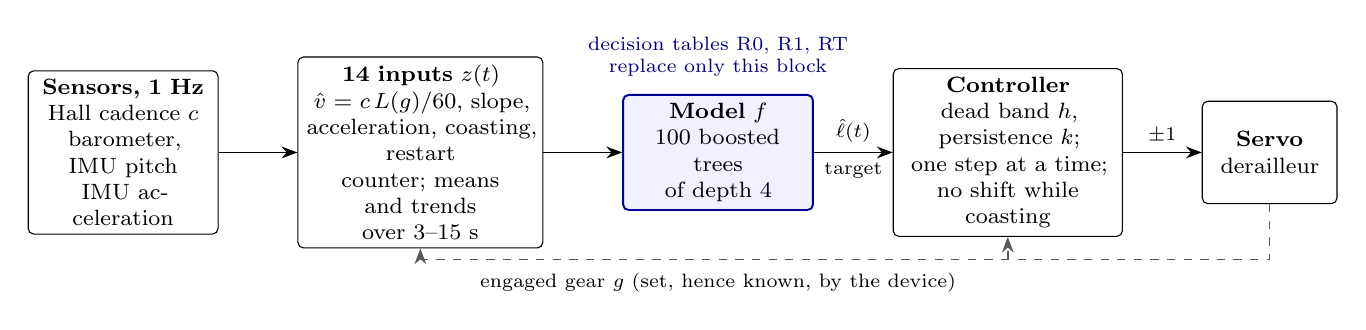
\begin{tikzpicture}[
  font=\footnotesize, node distance=4mm and 10mm,
  box/.style={draw, rounded corners=2pt, align=center, minimum height=13mm, inner sep=3pt, fill=white},
  learned/.style={box, draw=blue!60!black, fill=blue!6, line width=0.7pt},
  arr/.style={-{Stealth[length=2mm]}, line width=0.5pt},
  fb/.style={-{Stealth[length=2mm]}, line width=0.5pt, dashed, gray!70!black}]
\node[box, text width=2.2cm] (sens) {\textbf{Sensors, 1 Hz}\\ Hall cadence $c$\\ barometer, IMU pitch\\ IMU acceleration};
\node[box, text width=2.9cm, right=of sens] (feat) {\textbf{14 inputs $z(t)$}\\ $\vhat = c\,L(g)/60$, slope,\\ acceleration, coasting,\\ restart counter; means\\ and trends over 3--15~s};
\node[learned, text width=2.2cm, right=of feat] (model) {\textbf{Model $f$}\\ 100 boosted trees\\ of depth 4};
\node[box, text width=2.7cm, right=of model] (ctrl) {\textbf{Controller}\\ dead band $h$, persistence $k$;\\ one step at a time;\\ no shift while coasting};
\node[box, text width=1.5cm, right=of ctrl] (servo) {\textbf{Servo}\\ derailleur};
\draw[arr] (sens) -- (feat);
\draw[arr] (feat) -- (model);
\draw[arr] (model) -- node[above, font=\scriptsize]{$\lhat(t)$} node[below, font=\scriptsize]{target} (ctrl);
\draw[arr] (ctrl) -- node[above, font=\scriptsize]{$\pm 1$} (servo);
\coordinate (low) at ($(servo.south)+(0,-7mm)$);
\draw[fb] (servo.south) -- (low) -- (low -| feat.south) -- (feat.south);
\draw[fb] (low -| ctrl.south) -- (ctrl.south);
\node[font=\scriptsize, below=0.5mm of low -| model.south] {engaged gear $g$ (set, hence known, by the device)};
\node[font=\scriptsize, align=center, text=blue!50!black, above=1mm of model] {decision tables R0, R1, RT\\ replace only this block};
\end{tikzpicture}
\caption{Decision chain of the retained approach. The engaged gear enters only the computation of speed and the controller; since $c^P L(g^P) = c\,L(g^*)$, the inputs, and hence the model, are the same whatever gear the policy has chosen: the closed loop runs through the controller only.}
\label{fig:pipeline}
\end{figure*}

\subsection{From events to a target gear}
Let $\ell^*(t) = \log L\big(g^*(t)\big)$ denote the log-development of the rider's gear. The model estimates its value $H$ seconds ahead from the device's inputs $z(t)$, and the controller $C$ produces the next gear:
\begin{align}
\lhat(t) &= f_\theta\big(z(t)\big) \approx \mathbb{E}\big[\ell^*(t+H) \mid z(t)\big], \\
g(t+1) &= C\big(g(t),\ \lhat(t-k+1), \dots, \lhat(t)\big).
\end{align}
The shift event of Section~\ref{sec:event} is the discrete derivative of this target: $a(t) \neq 0$ exactly when $\ell^*$ jumps. Learning the level and letting the controller differentiate it changes the nature of the learning problem.

\emph{Imbalance disappears from the target (D2).} The target exists at every second. The most frequent gear covers about 30\pct{} of a ride on average (21 to 51\pct{} depending on the ride), and four to eight gears each cover at least 5\pct{}. Every second now carries a direct statement, ``in this state the rider wants this development'', where the classifier only saw ``no shift here''.

\emph{Timing ambiguity moves to the boundaries (D3).} The conditional expectation of the gear given the state is well defined and concentrated within about one step. Uncertainty about the instant only matters near the boundary between two gears, where the controller's dead band absorbs it.

\emph{The learned part leaves the loop (D4).} The target is defined without the current gear, and the inputs exclude it too. Even the derived speed is unaffected: by~\eqref{eq:replay}, $c^P(t)\,L\big(g^P(t)\big) = c(t)\,L\big(g^*(t)\big)$ whatever gear the policy selects. The model therefore sees the same inputs whether the rider or the policy chooses the gears; the closed loop runs through the controller only, a small hand-designed component whose dynamics are known.

\emph{Bicycles become comparable.} A development in metres per revolution means the same thing on every drivetrain; the logarithm makes the step between neighbouring gears roughly constant (0.05 to 0.15).

\emph{Looking ahead is possible, but buys little.} The horizon $H$ lets the model aim at the gear the rider will want a few seconds later. From past signals alone, however, that gear is barely more predictable than the current one; Section~\ref{sec:timing} shows that $H$ hardly changes the result.

The rarity of decisions does not vanish; it moves to the controller, where it becomes two design parameters chosen under a constraint on shift rate, instead of a statistical bias to be compensated in the loss. What remains is a milder imbalance of situations: steep climbs and high speeds are rare in the data, and the model is less accurate there.

\subsection{Inputs}
The model receives 14 inputs, all computable on the device (C2) and all defined in seconds, so that they can be refreshed every 0.5~s without retraining (Table~\ref{tab:inputs}). History enters through moving averages and differences over 3 to 15~s, which is how the model compensates for the missing torque (D1). Three quantities are deliberately absent. The current gear and the raw cadence would let the model learn ``keep the current gear'', which is right 97\pct{} of the time and useless; cadence enters only through $\vhat$, which does not depend on the gear chosen. Torque and power are excluded by C1.

\begin{table}[t]
\centering
\caption{Inputs of the target models.}
\label{tab:inputs}
\setlength{\tabcolsep}{3pt}
\begin{tabular}{@{}lL{3.0cm}L{2.9cm}@{}}
\toprule
Group & Inputs & Device source \\
\midrule
Speed & $\vhat$; means over 5 and 10~s; changes over 3 and 8~s & cadence $\times$ development of the engaged gear; IMU while coasting \\
Slope & value; means over 5 and 15~s & barometer or IMU pitch \\
Acceleration & value; means over 3 and 5~s & IMU, gravity removed \\
Coasting & flag; share of the last 5~s & Hall sensor ($c < 15$~rpm) \\
Restart & seconds since pedalling resumed (cap 10) & Hall sensor \\
\bottomrule
\end{tabular}
\end{table}

\subsection{Model}
The model $f_\theta$ is an ensemble of 100 regression trees of depth at most four, trained by gradient boosting~\cite{xgboost}:
\begin{multline}
f_\theta(z) = F_0 + \eta \sum_{m=1}^{100} w_{m,\,q_m(z)},\\
\min_{\theta} \sum_t \tfrac{1}{2}\big(\ell^*(t+H) - f_\theta(z_t)\big)^2 + \sum_m \tfrac{\lambda}{2}\lVert w_m \rVert^2,
\end{multline}
where $q_m(z)$ is the leaf of tree $m$ reached by $z$, $w_{m,j}$ the value of leaf $j$ of tree $m$, and $\eta = 0.1$ the learning rate. Trees are added one at a time, each fitted to the residuals of the previous ones; the optimal value of a leaf is the regularised mean of the residuals it holds. The other hyperparameters were fixed in advance and not tuned: row subsampling 0.8, input subsampling 0.9, at least 20 seconds per leaf, $\lambda = 1$. Trained on the whole dataset, the model has 1,446 decision nodes and 1,546 leaves; a prediction walks 100 trees of depth four, that is at most 400 comparisons and 100 additions, with no normalisation of inputs and no runtime library (D7).

\subsection{Controller}
The controller shifts up one step when, for $k$ consecutive seconds and while the rider pedals, the target exceeds the current gear by more than half a step plus a margin $h$:
\begin{equation}
\begin{split}
\lhat(s) - \log L(g) \ \ge\ \big(\tfrac{1}{2} + h\big)\big(\log L(g+1) - \log L(g)\big),\\
s = t-k+1, \dots, t.
\end{split}
\end{equation}
It shifts down in the symmetric case and holds otherwise. Equivalently, gear $g$ is kept as long as the target development $\hat L = e^{\lhat}$ stays in the dead band
\begin{equation}
L(g)\Big(\frac{L(g-1)}{L(g)}\Big)^{\frac12+h} < \hat L < L(g)\Big(\frac{L(g+1)}{L(g)}\Big)^{\frac12+h}.
\end{equation}
A jump of several gears is executed one step at a time. The setting selected by the protocol is $H = 3$~s, $h = 0.6$ and $k = 3$~s: the target must go 10\pct{} of a step beyond the neighbouring gear for three seconds before the controller acts, which is what keeps reversals rare.

As an illustration, take a seven-speed ladder 3.94--4.46--5.11--5.65--6.37--7.18--7.78~m with the bicycle in 5.11~m; the dead band runs from 4.40 to 5.71~m. On the flat at 30~km/h the model aims at 5.94~m (Table~\ref{tab:map}), so after three seconds the controller selects 5.65~m: 88.5~rpm instead of 98. On a 3\pct{} climb at 20~km/h it aims at 3.99~m, so the controller steps down twice, three seconds apart, and stops at 4.46~m, whose lower threshold is 3.89~m: 75~rpm instead of 59.

% =====================================================================================
\section{Results}\label{sec:results}
% =====================================================================================
\subsection{Against decision tables}
The three decision tables share the controller of Section~\ref{sec:method} and differ from the model only in their target. Each sets a target cadence $c^*$, from which the target development is $\log(60\,\vhat / c^*)$, and their constants are fitted by least squares to the rider's cadence on the training rides. Fitted on the whole dataset, they read: $c^* = 81.4$~rpm for R0; $c^* = 81.8 - 69.2\,s$ for R1, where $s$ is the slope ($-0.69$~rpm per percent); and $c^* = 73.3 - 138.8\,s + 0.043\,P$ for RT, where $P$ = torque $\times$ angular velocity is the pedalling power ($+4.3$~rpm per 100~W). RT is the decision table that a torque sensor would allow.

\begin{table}[t]
\centering
\caption{Closed-loop replay, 14 tests, means weighted by duration.}
\label{tab:main}
\setlength{\tabcolsep}{2.2pt}
\begin{tabular}{@{}lcccccc@{}}
\toprule
Policy & Torque & $\pm1$ gear & Exact & Shifts/h & Rev. & Band \\
\midrule
Rider (reference) & -- & 100\pct & 100\pct & 95 & 4.7\pct & 81.4\pct \\
\textbf{Retained model} & no & \textbf{87.0\pct} & \textbf{47.4\pct} & 95 & 0.2\pct & 66.3\pct \\
RT: cadence, slope, torque & yes & 80.8\pct & 40.8\pct & 112 & 0\pct & 69.3\pct \\
R1: cadence and slope & no & 80.4\pct & 39.1\pct & 112 & 0\pct & 69.3\pct \\
R0: constant cadence & no & 78.8\pct & 38.0\pct & 115 & 0\pct & 69.1\pct \\
Event classifier (V) & no & 66.0\pct & 27.7\pct & 96 & 4.9\pct & 52.2\pct \\
Never shift & -- & 44.2\pct & 16.1\pct & 0 & -- & 34.1\pct \\
\bottomrule
\end{tabular}
\\[2pt]
\parbox{\columnwidth}{\footnotesize Rev.: shifts undone within 4~s. Band: pedalling time with cadence inside the rider's 10--90\pct{} deciles.}
\end{table}

The retained model agrees with the rider within one gear 87.0\pct{} of the time, against 80.8\pct{} for the best decision table, which is given the torque the product does without (Table~\ref{tab:main}). It shifts exactly as often as the rider and almost never reverses a shift. The advantage holds in both groups: 85.7\pct{} against at most 80.0\pct{} for the decision tables on the Inria rider (10.4~h), and 88.5\pct{} against at most 82.2\pct{} on the five other riders (8.5~h). Test by test, the model beats every decision table in 13 of 14 cases, with a median margin of 5.7 points over the best decision table of each test (Fig.~\ref{fig:margin}). If the tests were independent, 13 wins out of 14 would have a one-sided sign-test probability of 0.001 under the hypothesis of no difference; they are not fully independent (four tests share a rider, and half-ride tests come in pairs), so this figure is indicative.

\begin{figure}[t]
\centering
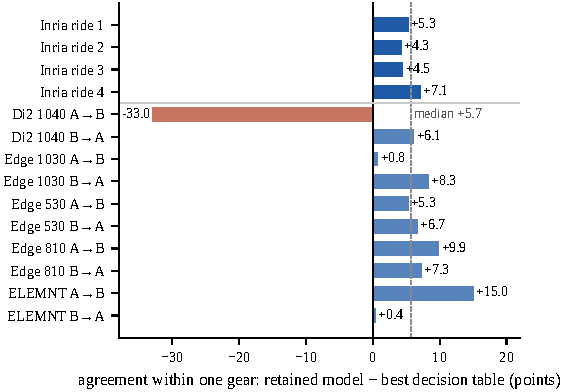
\includegraphics[width=\columnwidth]{fig_margin_per_test.pdf}
\caption{Margin of the retained model over the best decision table, test by test (A and B: first and second halves of a ride; darker bars: Inria rider).}
\label{fig:margin}
\end{figure}

Five findings deserve emphasis.
\emph{Torque adds almost nothing to a decision table:} from R1 to RT, overall agreement moves by only $+0.3$ points, and by between $-3.7$ and $+12.3$ points depending on the test. What a table lacks is not the instantaneous effort but the rider's habits, which the model learns from the recent history of speed and slope.
\emph{At equal calm, the model reacts faster:} to shift at most 1.2 times as often as the rider, the decision tables need a persistence of $k = 8$~s, and their shifts then come about 3~s after the rider's on average; with $k = 3$~s they would shift 180 to 190 times per hour. The model's target is steady enough for $k = 3$~s, and its shifts come about 1.7~s after the rider's (Section~\ref{sec:timing}).
\emph{The single failure is a data failure:} trained on 16 minutes of the Di2 ride, the model learns developments too large for the second half; it shifts 26 times per hour instead of 96 and drops to 51.9\pct{}. Trained on the other half, it reaches 92.1\pct{}. From 33 minutes of training upwards, every test is won.
\emph{Exact agreement stays low for every policy,} at best 47\pct{}: with nine or ten closely spaced sprockets, a one-step difference is barely felt, which is why agreement within one gear is the headline measure.
\emph{Imitating a rider is not the same as holding a cadence:} the decision tables keep slightly more pedalling time in the rider's cadence band (69\pct{} against 66\pct{}), because holding a cadence is exactly what they aim at. No policy reaches the rider's own 81\pct{}.

\subsection{Other statistical models}
Most of the gain comes from the reformulation, not from the model. To separate the two effects, five models were trained to predict the same target, with the same inputs, controller and selection protocol: a \emph{learned table} (median target in cells of 1~m/s of speed by 1\pct{} of 15-s mean slope, i.e.\ a shift schedule fitted to data, 289 cells of one byte), a \emph{linear regression} (ridge, standardised inputs), a \emph{small MLP} (two hidden layers of 16 units, early stopping), a \emph{random forest} (50 trees of depth at most 6) and the \emph{boosted trees}.

\begin{table}[t]
\centering
\caption{Same target, inputs, controller and protocol.}
\label{tab:models}
\setlength{\tabcolsep}{2.4pt}
\begin{tabular}{@{}lrccccc@{}}
\toprule
Model & Size & All & Inria & Single & Wins & Shifts/h \\
\midrule
\textbf{Boosted trees} & 13.5~KB & \textbf{87.0\pct} & 85.7\pct & \textbf{88.5\pct} & \textbf{13/14} & \textbf{95} \\
Small MLP & 2.2~KB & 86.8\pct & \textbf{86.7\pct} & 87.0\pct & 11/14 & 108 \\
Random forest & 31.4~KB & 85.8\pct & 84.9\pct & 86.9\pct & 11/14 & 107 \\
Linear regression & 172~B & 84.8\pct & 83.0\pct & 87.0\pct & 12/14 & 97 \\
Learned table & 289~B & 82.0\pct & 80.8\pct & 83.4\pct & 7/14 & 100 \\
Event classifier & 8.3~KB & 66.0\pct & 75.5\pct & 54.5\pct & 1/14 & 96 \\
\bottomrule
\end{tabular}
\\[2pt]
\parbox{\columnwidth}{\footnotesize Agreement within one gear. Wins: tests won against the best decision table. Sizes: medians over the 14 trained models, counting 8 bytes per tree node and 4 per float.}
\end{table}

A linear regression of 172 bytes on the 14 inputs already beats every decision table, the torque-aware one included, on 12 of 14 tests; nonlinear models add about two more points (Table~\ref{tab:models}, Fig.~\ref{fig:size}). The boosted trees and the MLP are statistically indistinguishable: the trees win 8 of the 14 paired tests; the MLP is ahead on the Inria rider (86.7\pct{} against 85.7\pct{}) and behind on short training sets (87.0\pct{} against 88.5\pct{}). The learned table, which is what a shift schedule fitted to data would be, gains only 1.2 points over the torque-aware decision table: a two-dimensional map of speed and slope cannot carry what the averages, trends and restart counter carry.

\begin{figure}[t]
\centering
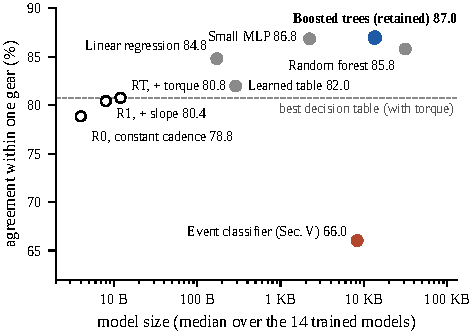
\includegraphics[width=\columnwidth]{fig_accuracy_vs_size.pdf}
\caption{Agreement within one gear against model size (log scale), 14 tests. Hollow: decision tables. Every model that predicts the target gear sits above the best decision table; the event classifier, which predicts shifts, sits far below it.}
\label{fig:size}
\end{figure}

\subsection{What sets the timing of shifts}\label{sec:timing}
The persistence $k$, not the horizon $H$, sets the timing of shifts (Table~\ref{tab:timing}). With $h = 0.6$ and $k = 3$~s fixed, sweeping $H$ from 0 to 8~s changes agreement within one gear by less than half a point (87.1 to 87.5\pct{}), and the mean delay of the policy's shifts behind the rider's only from 2.1 to 1.5~s. Sweeping $k$ instead moves that delay from 1.0~s ($k = 1$, at the cost of 140 shifts per hour and 4.4\pct{} reversals) to 2.4~s ($k = 5$). The policy therefore follows the rider by about two seconds rather than anticipating; its advantage over the decision tables lies in how steady a target it provides. Making downshifts more reactive than upshifts ($k = 1$~s down, 3~s up) brings the median downshift delay from 3 to 1~s and raises agreement to 88.0\pct{}, for 113 shifts per hour, just below the 1.2$\times$ limit. Delays are measured against reconstructed shift times, themselves accurate to about $\pm 3$~s (Section~\ref{sec:data}), and are indicative only.

\begin{table}[t]
\centering
\caption{Shift timing, 14 tests, fixed settings (no selection).}
\label{tab:timing}
\setlength{\tabcolsep}{3pt}
\begin{tabular}{@{}lcccc@{}}
\toprule
Policy and setting & $\pm1$ gear & Shifts/h & Rev. & Mean delay \\
\midrule
Model, $H{=}0$, $k{=}3$ & 87.1\pct & 92 & 0.7\pct & +2.1~s \\
Model, $H{=}3$, $k{=}3$ & 87.3\pct & 93 & 0.5\pct & +1.7~s \\
Model, $H{=}8$, $k{=}3$ & 87.1\pct & 96 & 0.6\pct & +1.5~s \\
Model, $H{=}3$, $k{=}1$ & 89.3\pct & 140 & 4.4\pct & +1.0~s \\
Model, $H{=}3$, $k{=}5$ & 85.5\pct & 74 & 0\pct & +2.4~s \\
Model, $H{=}3$, $k$ 3 up / 1 down & 88.0\pct & 113 & 1.1\pct & +1.4~s \\
RT, $h{=}0.3$, $k{=}8$ (selected) & 80.8\pct & 112 & 0\pct & +3.2~s \\
RT, $h{=}0.6$, $k{=}3$ & 82.9\pct & 189 & 2.2\pct & +1.4~s \\
\bottomrule
\end{tabular}
\\[2pt]
\parbox{\columnwidth}{\footnotesize Delay: mean lag of the policy's shifts behind the rider's same-direction shifts within $\pm 10$~s; positive = late.}
\end{table}

\subsection{What the model learned}
Three quarters of the model's error reduction comes from speed and one fifth from slope: speed inputs carry 75.6\pct{} of the total split gain, slope 19.0\pct{}, acceleration 2.6\pct{}, the restart counter 2.5\pct{} and coasting 0.4\pct{}. The resulting map (Table~\ref{tab:map}) resembles the shift schedule of an automatic car gearbox, but learned from riders. The development grows with speed, but less than proportionally, so the implied cadence rises with speed, from 37 to 87~rpm on the flat: riders spin faster when they go faster, which no constant-cadence table can reproduce. At equal speed, climbing calls for a smaller gear (84~rpm instead of 69 at 20~km/h on a 3\pct{} slope), and descending for large gears and low cadence. Beyond 3\pct{} the map barely changes, a sign of how few steep climbs the data contain rather than a physical law.

\begin{table}[t]
\centering
\caption{Learned target development (m) and resulting cadence (rpm) at constant speed and slope, zero acceleration, after 10~s of pedalling.}
\label{tab:map}
\setlength{\tabcolsep}{2.2pt}
\begin{tabular}{@{}lcccccc@{}}
\toprule
Slope & 10~km/h & 15~km/h & 20~km/h & 25~km/h & 30~km/h & 35~km/h \\
\midrule
$-5$\pct & 5.39 $\cdot$ 31 & 5.86 $\cdot$ 43 & 6.02 $\cdot$ 55 & 6.58 $\cdot$ 63 & 7.29 $\cdot$ 69 & 8.06 $\cdot$ 72 \\
0\pct & 4.50 $\cdot$ 37 & 4.76 $\cdot$ 53 & 4.85 $\cdot$ 69 & 5.35 $\cdot$ 78 & 5.94 $\cdot$ 84 & 6.70 $\cdot$ 87 \\
$+3$\pct & 3.24 $\cdot$ 51 & 3.49 $\cdot$ 72 & 3.99 $\cdot$ 84 & 5.04 $\cdot$ 83 & 5.62 $\cdot$ 89 & 6.38 $\cdot$ 92 \\
$+6$\pct & 3.20 $\cdot$ 52 & 3.54 $\cdot$ 71 & 4.19 $\cdot$ 80 & 5.30 $\cdot$ 79 & 5.89 $\cdot$ 85 & 6.57 $\cdot$ 89 \\
\bottomrule
\end{tabular}
\end{table}

\subsection{Without personalisation}
The within-rider protocol mirrors the product, which learns its own rider. To see what personalisation contributes, every policy was also trained on five riders and tested on the sixth, with decision parameters selected by an inner leave-one-rider-out over the training riders. The learned policy then loses its advantage: 72.5\pct{} agreement within one gear, against 75.2\pct{} for the torque-aware table and 73.5\pct{} for the constant-cadence one. It beats every decision table on two riders out of six and collapses on the shortest ride (Di2, 28.7\pct{}). The decision tables lose about 5 points against the within-rider protocol, the learned policy 14.5. What the model learns is a rider's habits, and they do not transfer.

% =====================================================================================
\section{Embedded Implementation}\label{sec:embedded}
% =====================================================================================
The retained policy is implemented in plain C99 for the nRF52840, in three modules with no heap, no recursion and no runtime library: the input computation (ring buffers of 16 samples), the tree inference and the controller.

\emph{Model layout.} Each tree is stored as a complete binary tree of depth four, so no child pointers are needed: node $i$ has children $2i+1$ (input below the threshold) and $2i+2$, the convention of XGBoost. A branch that training pruned early is padded with thresholds set to $+\infty$ and repeated leaf values. Each tree then takes 15 single-precision thresholds, 15 one-byte input indices and 16 leaves, that is 139 bytes, and 13,904 bytes for the 100 trees and the bias. A prediction is exactly 400 comparisons and 100 additions, whatever the input, which makes the timing of the control loop predictable.

\emph{Footprint.} Compiled with \texttt{arm-none-eabi-gcc} 14.2 for the Cortex-M4F (\texttt{-Os}, hardware single-precision floating point), the library occupies 14,944 bytes of flash: 13,904 bytes of model constants and 1,040 bytes of code (Table~\ref{tab:footprint}). Its state, the input buffers and the controller, takes 316 bytes of RAM. That is 1.5\pct{} of the flash and 0.1\pct{} of the RAM of the board.

\begin{table}[t]
\centering
\caption{Firmware footprint on the Cortex-M4F (\texttt{-Os}).}
\label{tab:footprint}
\setlength{\tabcolsep}{4pt}
\begin{tabular}{@{}lrr@{}}
\toprule
Module & Flash (B) & RAM (B) \\
\midrule
Tree constants (100 trees, depth 4) & 13,904 & 0 \\
Tree inference & 116 & 0 \\
Inputs (14, ring buffers) & 520 & 224 \\
Controller & 404 & 92 \\
\midrule
Total & 14,944 & 316 \\
\bottomrule
\end{tabular}
\end{table}

\emph{Verification.} A host test replays three rides (14,261 seconds) through the C library and compares it with the Python reference. The C inference reproduces the predictions exactly on the Python inputs; the C inputs differ from the Python ones by at most $3\times10^{-6}$; fed with the Python targets, the C controller selects exactly the same gear at every second. Run entirely in C as on the bicycle, measuring the cadence produced by its own gear, the policy selects the same gear as the Python replay on 99.7\pct{} of the seconds, and stays within one gear of it at every second. The integration with the sensors and the servo is provided as an example sketch, but has not been tested on the bicycle, since the prototype is no longer available.

% =====================================================================================
\section{Discussion}\label{sec:discussion}
% =====================================================================================
\subsection{Why boosted trees}
Between the boosted trees and the MLP, accuracy alone does not decide; the choice rests on how each behaves in the regime the product will face. \emph{Consistency:} the trees beat the best decision table on 13 of 14 tests, the MLP on 11; the one test the trees lose, every learned model loses (43 to 58\pct{} after 16 minutes of training). \emph{Little data:} a new user brings an hour of riding, not ten (D6). On the five single-ride riders the trees reach 88.5\pct{}, against 87.0\pct{} for both the MLP and the linear regression; they also need no validation split to stop training, whereas the MLP's early stopping carves one out of an already short ride. \emph{Riding behaviour:} the trees shift 95 times per hour, the rider's own rate, and reverse 0.2\pct{} of their shifts; the MLP shifts 108 times per hour and reverses four times as often. For a rider, an unnecessary shift is the most noticeable error. \emph{Deployment (D7):} the trees take raw inputs, with no per-input mean and variance to store and keep consistent between training and firmware; their inference is a fixed sequence of comparisons; their split gains give the reading of Table~\ref{tab:map}.

The MLP remains a credible alternative where memory is scarce: it is six times smaller and slightly better on the data-rich rider. The linear regression, at 172 bytes, is the natural fallback for a user who has not yet recorded enough to train a richer model. The random forest is dominated: larger than the boosted trees and less accurate on 13 of 14 tests. One property of trees cuts both ways: their prediction is constant beyond the last split, so they never extrapolate wildly outside the training range, but for the same reason they cannot extend the map to slopes steeper than the data contain.

\subsection{What the proof of concept shows}
On the closest public equivalent of the prototype's data, the answer to the question of Section~\ref{sec:question} leans towards the learned policy. Using only what the device measures, without torque, it agrees with the rider within one gear 87.0\pct{} of the time in closed-loop replay, against 80.8\pct{} for a decision table given the pedalling torque; it wins 13 of 14 within-rider tests, shifts as often as the rider, almost never reverses a shift, and fits in 14.9~KB of flash. Each difficulty has a counterpart in the design (Table~\ref{tab:difficulties}).

\begin{table}[t]
\centering
\caption{The difficulties of Section~\ref{sec:difficulties} and how they are resolved.}
\label{tab:difficulties}
\setlength{\tabcolsep}{3pt}
\begin{tabular}{@{}L{1.85cm}L{5.0cm}l@{}}
\toprule
Difficulty & Resolution & Sec. \\
\midrule
D1 Partial observability & averages and trends over 3--15~s stand in for effort; torque adds 0.3 points to a table & VI, VII \\
D2 Rare decisions & the target gear exists at every second; rarity becomes two controller parameters & VI \\
D3 Ambiguous timing & learn the level, not the instant; the dead band absorbs boundary uncertainty & VI \\
D4 Closed loop & inputs do not depend on the gear chosen; every policy judged in closed-loop replay & IV, VI \\
D5 No first-party data & public rides restricted to device quantities, labels validated on real Di2 shifts & III \\
D6 Little data & 14 inputs, 100 shallow trees; every test won from 33 minutes of training & VII \\
D7 Embedded budget & 14.9~KB of flash, 316~B of RAM, fixed 400 comparisons & VIII \\
D8 No prototype & replay with the cadence recomputed from the policy's own gear; C port verified against it & IV, VIII \\
\bottomrule
\end{tabular}
\end{table}

Two findings reach beyond this dataset. First, the formulation matters more than the model: on the same inputs, a 172-byte linear regression of the target gear beats every decision table, while a boosted classifier of shift events loses to the simplest one. Second, the premise of the product holds up: torque adds almost nothing to a decision table, and what a table lacks, the rider's habits and a target steady enough to act on quickly, a model can learn from the recent past of signals the device already has.

These results point to a learned policy choosing gears better than a decision table, but they do not prove it. Without a test on the bicycle, the margin cannot be confirmed: the labels are reconstructed and the closed loop is simulated. Some confidence is nonetheless warranted. All policies share the same controller, the same mechanical rules and the same labels, so label noise penalises them alike; and the main assumption of the replay, that speed does not depend on the gear chosen, holds best for the policy that stays closest to the rider, which is the learned one. It is therefore reasonable to assume that on the bicycle the learned policy would be at least as good as a decision table, with the advantage measured here as the more likely outcome.

\subsection{Limits of the model}
\emph{Agreement is measured against noisy labels:} the rider's gear is reconstructed and correct 84\pct{} of the pedalling time, and exact agreement stays below 50\pct{} for every policy; the 87.0\pct{} figure compares policies on equal terms, it is not the accuracy a rider would perceive.
\emph{It needs data before it helps:} with 16 minutes of training it falls to 51.9\pct{}, far below the decision tables; a product would start from a decision table or from the linear regression, and switch to the learned model once a user has recorded about half an hour.
\emph{Rare situations are poorly learned:} steep climbs and high speeds are scarce in the data, and beyond 3\pct{} of slope the learned map barely changes.
\emph{It is personal:} trained on other riders, it falls to 72.5\pct{}, below the torque-aware decision table (75.2\pct{}); the product must learn each user, which makes the previous point a real constraint.
\emph{It imitates gears, not comfort:} it keeps less pedalling time in the rider's cadence band than the decision tables (66\pct{} against 69\pct{}), and no policy approaches the rider's own 81\pct{}.
\emph{It follows rather than anticipates:} its shifts come about 1.7~s after the rider's on average, a delay set by the controller's persistence rather than by the horizon; the model knows nothing of the road ahead, and the slope it receives here lags the terrain by several seconds.

\subsection{Limits of the method}
\emph{Reconstructed, not recorded:} the data come from six ordinary riders on head units, not from my team riding the prototype; the labels are gear sequences inferred from the speed-to-cadence ratio rather than shift commands, and the inference was validated on a single Di2 ride of 33 minutes.
\emph{Different sensors:} cadence is sampled at 1~Hz instead of once per revolution; the slope comes from a head unit's altitude, which lags the terrain, rather than from a barometer or the IMU pitch, which would respond almost at once but with vibration noise; acceleration is a derivative of speed; speed while coasting is read from the record rather than integrated from the IMU, which drifts. The device's inputs will be noisier, and the raw IMU signals the prototype offers (vibration, lean, standing) were not used at all.
\emph{Simulated closed loop:} the replay holds speed fixed whatever gear the policy selects; this is sound while the policy stays close to the rider, but it ignores how a rider reacts to a gear they did not choose: pushing harder, slowing down, or overriding.
\emph{Simple references:} the decision tables fit a linear target cadence; a hand-tuned schedule, fuzzy rules~\cite{fuzzy} or a system that learns from the rider's corrections~\cite{qauto} would be stronger baselines, and the margin over them is unknown.
\emph{Little, dependent evidence:} 18.9 hours, six riders and 14 tests, four of which share a rider and ten of which come in pairs; significance levels are indicative only, and the decision parameters were selected on a single rider.
\emph{Mechanics left out:} servo latency, shifting under load and chain wear are outside the simulation; timing a shift to a moment of light pedal load, a separate use a torque signal could have, is not addressed.

% =====================================================================================
\section{Conclusion and Outlook}
% =====================================================================================
This extension of AutoGear set out to test, without the prototype and without its data, whether a statistical model can choose gears better than a decision table on a bicycle that has no torque sensor. Rebuilding the missing dataset from public sources and replaying every policy in closed loop, the answer is positive on that data: a regression of the target gear, coupled with a hysteresis controller, agrees with the rider within one gear 87.0\pct{} of the time against 80.8\pct{} for a torque-aware decision table, and runs in 14.9~KB of flash on the target microcontroller. The decisive step was not the choice of model but the change of formulation, from predicting rare and noisy shift events to regressing a target that exists at every second and keeps the learned part out of the loop.

The proof of concept turns the original plan into a narrower, testable one. A first-party study would record with the prototype, whose servo state gives exact gear labels and whose IMU and barometer give a faster slope than the altitude used here. It would start each user on the linear regression or a decision table and switch to the boosted trees after about half an hour of riding; make downshifts more reactive than upshifts, since a late downshift at the foot of a climb is the costly error; and close the loop for real, collecting the rider's overrides as corrections in the manner of DAgger~\cite{dagger}, so that the model and controller described here are judged on the bicycle rather than in replay.

\section*{Acknowledgment}
The Shifter Pro prototypes were designed and built within the AutoGear team, with Corentin Hesry, Vincent Lucien and Maxime Poulain; the embedded electronics were built with Vincent Lucien. The extension reported here, from the reconstruction of the dataset to the firmware library, was carried out by the author after the project.

\section*{Code and Data Availability}
The data pipeline, experiments, firmware library and the scripts that produce every number and figure of this report are available at \url{\repourl}. The public source files are downloaded from their original repositories at pinned commits and are not redistributed.

\bibliographystyle{IEEEtran}
\bibliography{refs}

\end{document}
